\chapter[SCP-031 爱为何物?]{
    SCP-031 What is Love?\\
    SCP-031 爱为何物?
}

\label{chap:SCP-031}

\begin{figure}[H]
    \centering
    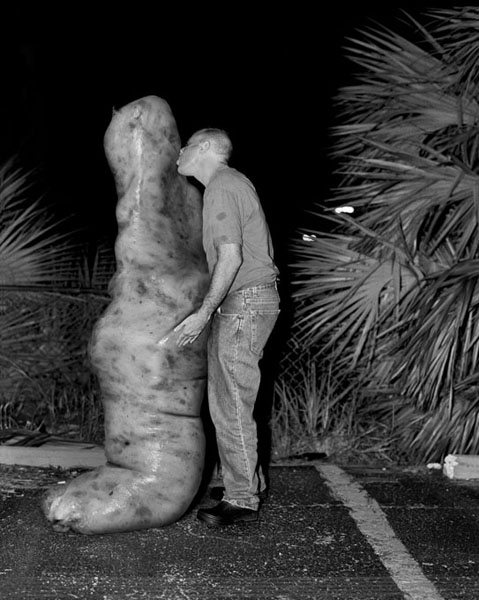
\includegraphics[width=0.5\linewidth]{images/SCP.031.jpg}
    \caption*{在最初的收容中被发现的SCP-031的照片。}
\end{figure}

\bb{项目编号:}SCP-031

\bb{项目等级:}Safe

\bb{特殊收容措施:}SCP-031应收容于位于77号站点的Safe级SCP侧楼的标准\dd{类人对象}收容室。与SCP-031互动的人员不得直接观测它,并应通过安装在每间房间中的内部通话系统与实验者交流。收容室应由监护员工每周打扫一次,打扫员工须戴遮光护目镜以削弱SCP-031的影响。

\bb{描述:}SCP-031是一个无定形生物,重75千克。SCP-031能以每小时3千米的速度移动,移动时产生一条油迹。对象仅能进行基本的移动。对回收到的组织样品的测试显示SCP-031成分中至少有人类的肌肉和表皮组织。SCP-031能够模仿任何音高和语气的人类话语,但目前不清楚SCP-031生物学上如何发出声音的。

直接观察SCP-031的对象会视其为自己认识并且曾经爱慕过的一个人。意识到自己被观察后,SCP-031将自称是前文所述之人且由于过去的某个事件而一贫如洗。SCP-031会以此事试图说服对象允许它在身边呆上较长的一段时间,直到它的生活能够安定下来。该效应对所有看见SCP-031的人有效,且研究尚未找到同时受SCP-031影响人数的上限。

在观察住所后,SCP-031将尝试与对象开始一段恋爱关系,如果这段关系成功建立,SCP-031将在对象家住下。当SCP-031开始影响额外的对象时,它会劝说他们打消恋爱的念头。几起SCP-031开始积极地同时影响多个对象的事例已被记录,最后竟然有一个巢包含至少18个不同酒店房间,这些房间内包括了不同对象和部分的SCP-031。

SCP-031是在{[}编辑]的骚动后,由于警察的口供自相矛盾而被发现收容的。多名对象汇报了关于SCP-031外貌的相差甚远的看法,开始的平民单位也遭到影响。不过,记忆消除剂和吸入式镇静剂的大范围使用让所有受影响对象平静下来,之后MTF(机动特遣队)-Psi-7从SCP-031所居住的酒店中将其成功收容。自11\slash 16\slash 1958起,SCP-031被分级为Safe。

\bb{附录:}研究发现无恋者对象不受SCP-031影响。然而,所有这类对象均称SCP-031是一个娇小丰满的人形,外貌被SCP-031的体内逸散的黑烟所掩盖。需后续测试以解释此原因。
